\setcounter{chapter}{-1}
\chapter{Puzzles and anecdotes}\label{chap:anecdot}



You have probably heard that for topologists, \textit{two shapes are the same if
one can be turned into the other by stretching and squeezing} (without ripping, piercing, gluing, and so on).

This statement is neither precise nor correct, but it helps build intuition.
So, imagine an object made from endlessly stretchy material that can be twisted and pulled like chewing gum;
if you can get one shape from another, then they have the same topology.
Note that the size plays no role.

\begin{figure}[!ht]
\centering
\includegraphics{mppics/pic-110}
\end{figure}

\begin{wrapfigure}{r}{47 mm}
\vskip-2mm
\centering
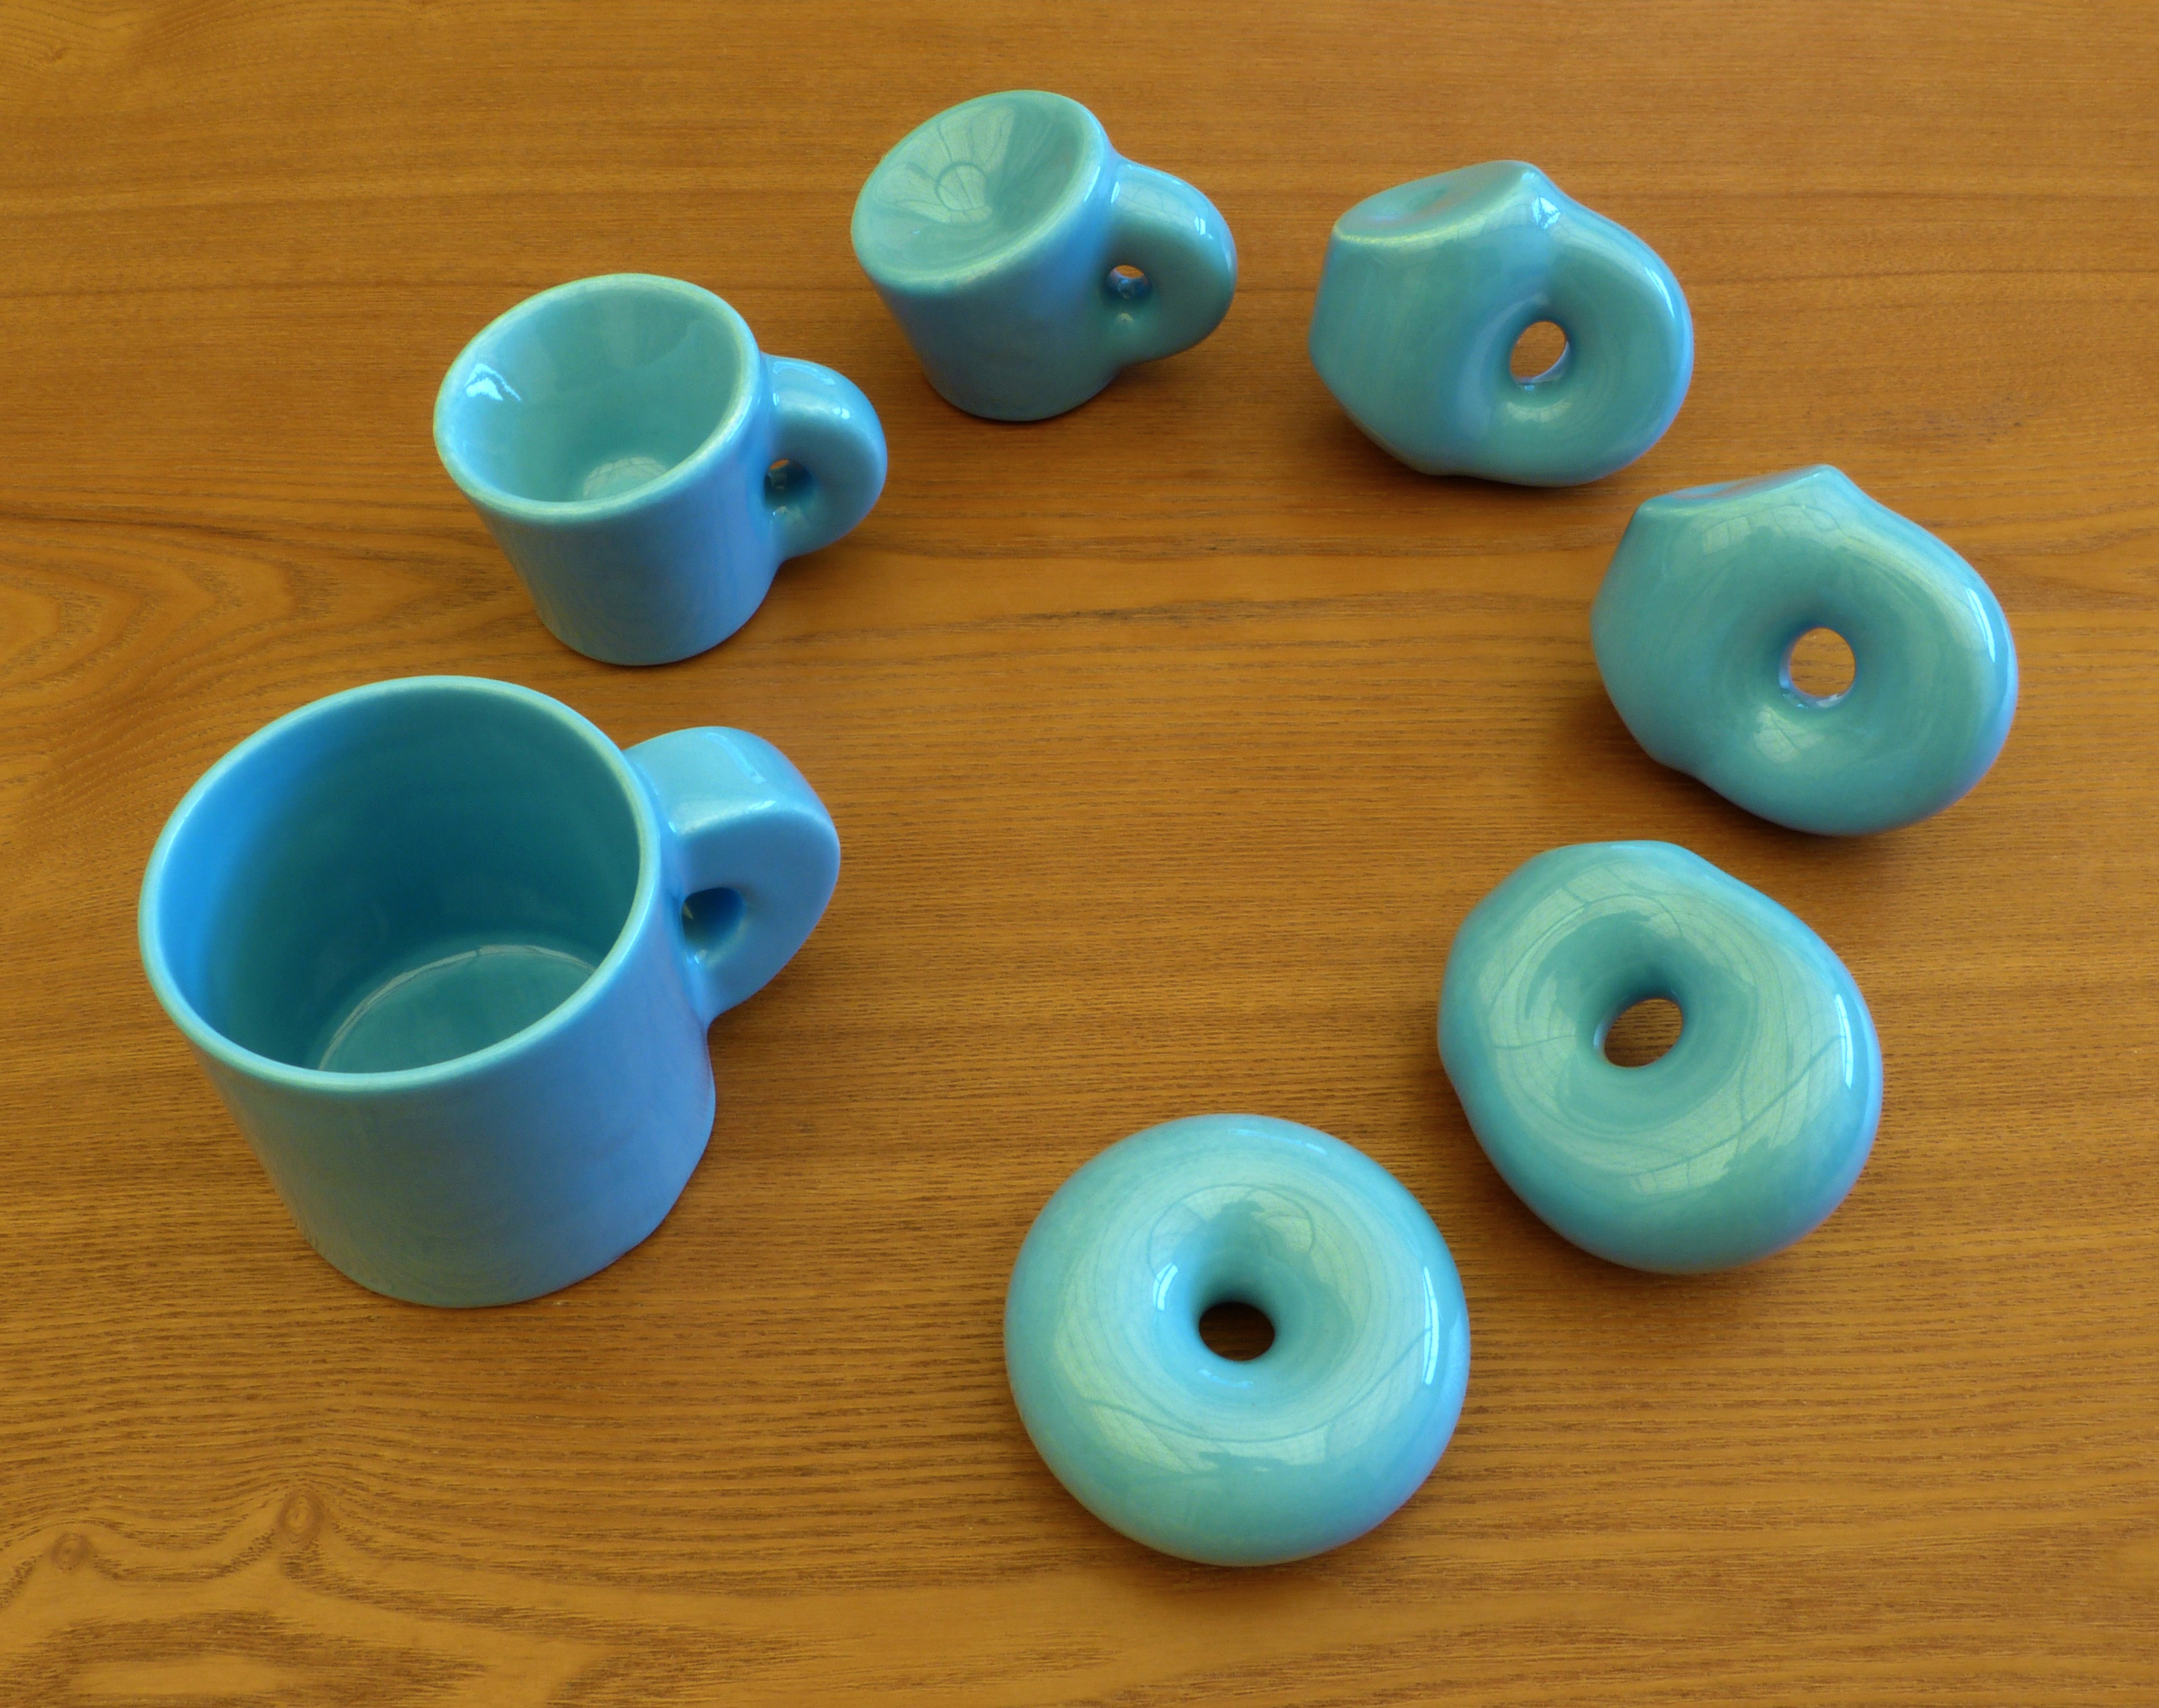
\includegraphics[scale=.035]{pics/mug-to-donut}
\end{wrapfigure}

The picture above suggests that a square and a disc have the same topology.
It might be more impressive to see that a donut is topologically equivalent to a coffee mug.
On the other hand, a disc and an annulus are topologically different.
It might be obvious, but this is a nontrivial statement
(it will follow from \ref{thm:pi1(S1)}).
So, at least not all shapes are topologically equivalent.

\begin{wrapfigure}[3]{r}{47 mm}
\vskip-4mm
\centering
\includegraphics{mppics/pic-120}
\end{wrapfigure}


\begin{thm}{Exercise}\label{ex:morning}
In the morning, a topologist looks at his clothes; there should be a T-shirt, a pair of pants, and socks.
Help him to identify each piece of clothing.
Which piece has a hole in it?

\end{thm}


\begin{thm}{Exercise}\label{ex:mug}
A topologist dropped his mug and noticed that the handle had snapped off.
``Its topology has changed,'' he thaut, ``but it can still be used for its intended purpose.''

He picked the mug up, turned it over, and said:
``Oh, I was wrong---the topology has not changed, but it is now impossible to use.''

What did he see?
\end{thm}

{

\begin{thm}{Exercise}\label{ex:finger-ring}
The topologist decided to fix the broken mug with superglue.
Being a rather clumsy person, he somehow managed to glue his index finger to his thumb---in fact, on both hands.
\begin{figure}[h!]
\centering
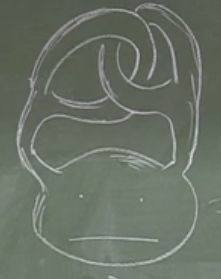
\includegraphics[scale=.3]{pics/1}
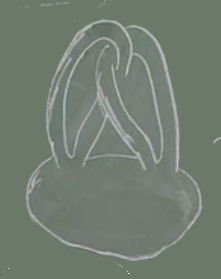
\includegraphics[scale=.3]{pics/2}
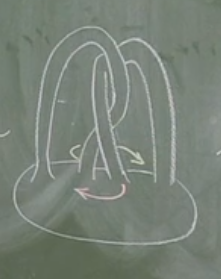
\includegraphics[scale=.3]{pics/3}
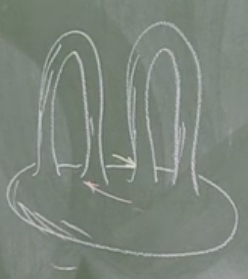
\includegraphics[scale=.3]{pics/4}
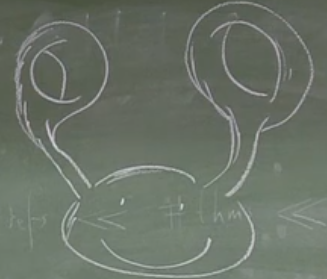
\includegraphics[scale=.3]{pics/5}
\end{figure}
Worse still, the finger rings he'd made were linked together.
But after some thinking and stretching he managed to separate the rings.

\begin{wrapfigure}{r}{19 mm}
\vskip-6mm
\centering
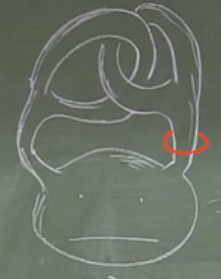
\includegraphics[scale=.3]{pics/1a}
\end{wrapfigure}

What would happen if he had a hair tie on his hand?
\end{thm}

At this point, you might think that topology has no practical value, and you are almost right, but it helps in solving the following puzzles;
these puzzles can also help you to start thinking topologically.

}

\begin{wrapfigure}{r}{25 mm}
\vskip-4mm
\centering
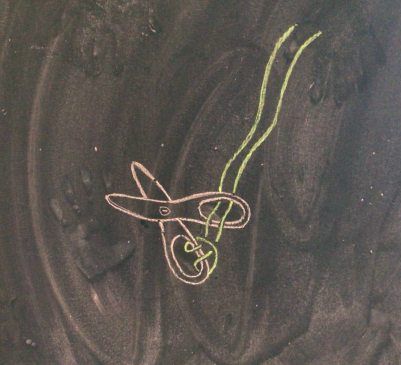
\includegraphics[scale=.2]{pics/scissors-bb}\\
\bigskip
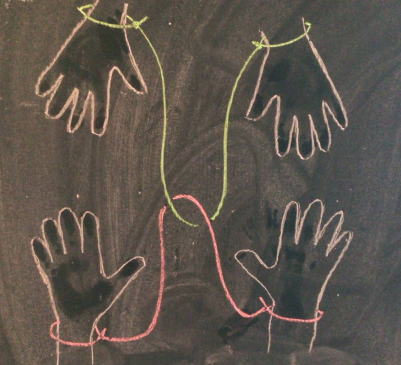
\includegraphics[scale=.2]{pics/4-hands}\\
\bigskip
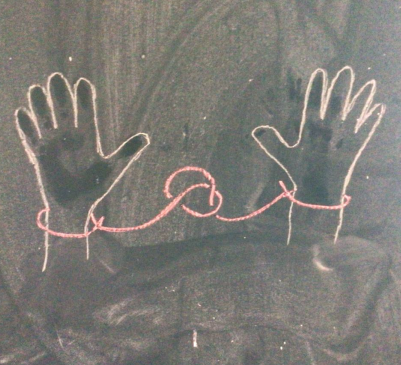
\includegraphics[scale=.2]{pics/2-hands}
\end{wrapfigure}

\begin{thm}{Exercise}\label{ex:scissors}

\begin{subthm}{ex:scissors:scissors}
Put a loop of cord thru the handles of a pair of scissors as shown.
Have someone hold the ends.
Try to get the scissors off without cutting the cord or releasing the ends.
\end{subthm}

\begin{subthm}{ex:scissors:4-hands}
Tie your hands together with a long cord;
then tie the hands of your friend in the same way, linking your cords, as shown.
Now try to get them apart without cutting the string or untying the knots.
\end{subthm}

\begin{subthm}{ex:scissors:2-hands}
If there is no friend nearby, try undoing the knot in the middle of the cord shown in the last picture.
Again, no cutting the string or untying the little knots.
\end{subthm}



\end{thm}


